\begin{figure}[h]
  \center
  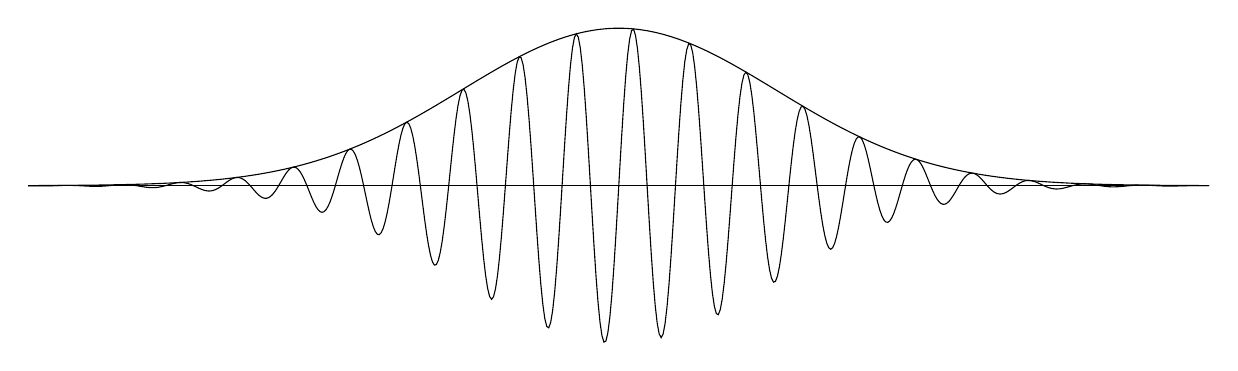
\begin{tikzpicture}
    % parametri
    \def\asse{15}
    \def\A{2}        % ampiezza
    \def\mu{0}       % centro
    \def\sigma{2}    % larghezza

    \def \gaussiana {\A*exp(-((\x-\mu)^2)/(2*\sigma^2))}
    \def \f {sin(500*\x)}
    \draw (-\asse/2, 0) -- (\asse/2, 0);

    \draw [domain = -\asse/2: \asse/2, samples=600] plot (\x , {\gaussiana});
    %\draw [domain = -\asse/2: \asse/2, samples=200] plot (\x , {-\gaussiana});

    \draw [domain = -\asse/2: \asse/2, samples=600] plot (\x , {\f*\gaussiana});

  \end{tikzpicture}
  \caption{Pacchetto d'onda gaussiano}
  \label{figure:_pacchetto d'onda}
\end{figure}
